A dobozba zárt részecske esetében két esetet kell vizsgálni a szemiklasszikus energiaszintek meghatározásához. Az első eset, amikor az energia $E < FL$, tehát a fordulópont a második fal elérése előtt van. Ebben az esetben a Maslov index $\frac{3}{4}$ \cite{brack:semiclassical} (2.4.1 fejezet). Az $x=0$ fordulópontban a szemiklasszikus hullámfüggvény $\frac{\pi}{4}$ fázist vesz fel, az $x=E/F$ fordulópontban pedig $\frac{\pi}{2}$ fázist vesz fel,
\begin{equation}
	\left(n+\frac{3}{4}\right)h=\oint p\,dq=2\int_0^{E/F}\sqrt{2m\left( E-Fx \right)}\,dx=\frac{4\sqrt{2m}}{3F}E^{3/2}.
	\label{semiclassicallevels:e1}
\end{equation}
A második eset amikor $E > FL$, ekkor a fordulópontok $0$-ban és $L$-ben vannak, és a Maslov index $1$. Mind az $x=0$, mind az $x=L$ fordulópontban $\frac{\pi}{2}$ fázis vesz fel a szemiklasszikus hullámfüggvény,
\begin{equation}
	\left(n+1\right)h=\oint p\,dq=2\int_0^{L}\sqrt{2m\left(E-Fx\right)}\,dx=\frac{4\sqrt{2m}}{3F}\left(E^{3/2}-\left(E-FL\right)^{3/2}\right).
	\label{semiclassicallevels:e2}
\end{equation}
\begin{figure}[H]
	\centering
	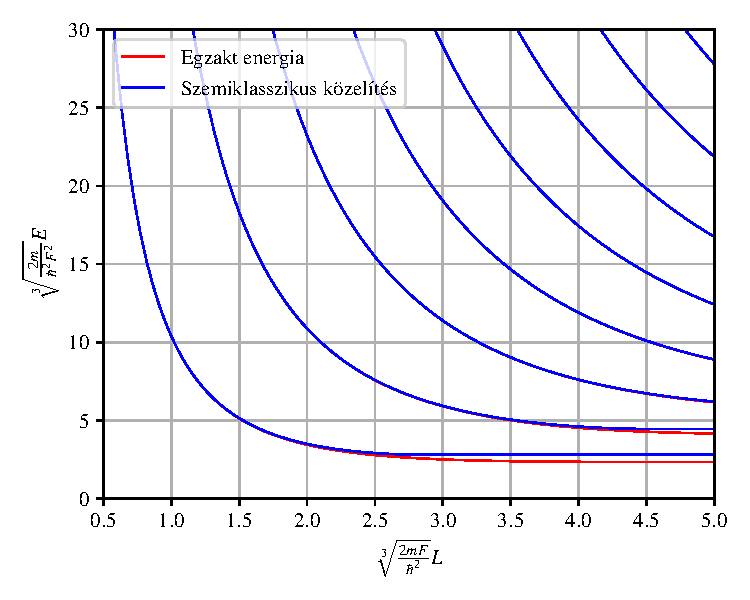
\includegraphics[scale=1]{./figs/energiaszintkozelites.pdf}
	\caption[Szemiklasszikus energiaszintek]{Az ábrán a szemiklasszikus energiaszintek összehasonlítása látható az egzakt energiaszintekkel. Ez az ábra is a $bE$ és $aL$ közötti relációt ábrázolja. A szemiklasszikus közelítés nagy kvantumszámok illetve ebben a esetben $E \gg FL$ esetén is pontos. Utóbbi oka, hogy ebben az esetben a potenciál elhanyagolható, és a potenciál nélküli végtelen potenciálgödör energiaszintjeit pedig a szemiklasszikus közelítés egzaktul megadja.}
	\label{semiclassicallevels:kozelites}
\end{figure}
Előfordulhat, hogy valamely $n$-re egyszerre van \eqref{semiclassicallevels:e1} és \eqref{semiclassicallevels:e2} egyszerre van megoldása, ahol $E$ a megfelelő tartományba esik. Ez azt jelenti, hogy a szemiklasszikus közelítés hibáján belül nem lehet meghatározni, hogy a valódi energiszint $FL$ felett, vagy alatt van. \Aref{semiclassicallevels:kozelites}. ábra az $E$-$L$ diagrammon szemlélteti a szemiklasszikus köelítés pontosságát. Két különböző esetben is pontos a szemiklasszikus közelítés. Nagy kvantumszámok esetében általánosságban is igaz, hogy pontos a szemiklasszikus közelítés. Ezen felül $E\gg FL$ esetében is pontos, ennek oka, hogy ilyenkor a lineáris potenciál elhanyagolható, viszont az így kapott problémát, a végtelen potenciálgödröt, a szemiklasszikus közelítés egzaktul írja le. \Aref{semiclassicallevels:allapotszam}. ábra szemlélteti a szemiklasszikus és egzakt állapotszámok viszonyát. A szemiklasszikus energiaszintekre vonatkozó egyenleteket minden esetben kézenfekvő az állapotok számának meghatározására használni, hiszen az egyenlet alapból $n$-re van rendezve a Maslov-indextől eltekintve. 
\begin{figure}[H]
	\centering
	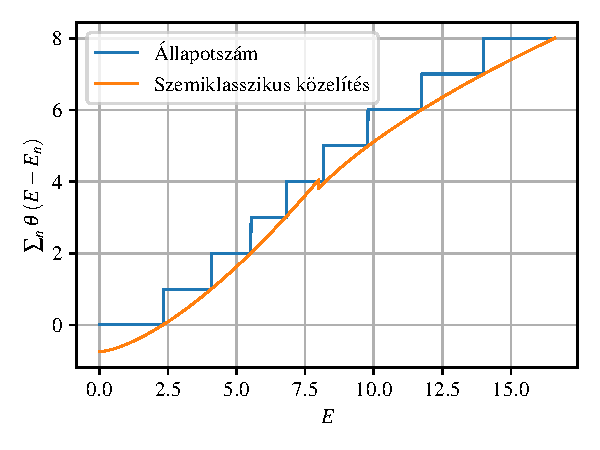
\includegraphics[scale=1]{./figs/allapotszam.pdf}
	\caption[Szemiklasszikus állapotszám]{A szemiklasszikus és egzakt energiaszintek összevetése. A kék vonal az egzakt energiák által meghatározott állapotszám. A narancssárga vonal pedig \aeqref{semiclassicallevels:e1} vagy \aeqref{semiclassicallevels:e2} ($E$ és $FL$ relációjától függően) egyenletekből kapott $n$ az energia függvényében.}
	\label{semiclassicallevels:allapotszam}
\end{figure}
Amennyiben $E \gg FL$ \aeqref{semiclassicallevels:e2} egyenleten a különbség az $E^{3/2}$ függvény deriváltjának segítségével helyettesíthető,
\begin{equation}
	(n+1)h \approx FL\frac{d}{dE}\left(\frac{4\sqrt{2m}}{3F}E^{3/2}\right)=2\sqrt{2m}E^{1/2}L.
\end{equation}
Átrendezve az egyenletet energiára a megszokott végtelen potenciálgödör energiaszintjeit kapjuk,
\begin{equation}
	E_n \approx \frac{(n+1)^2h^2}{8mL^2}.
\end{equation}
Ezeket az energiaszinteket \aref{semiclassicallevels:squarewell}. ábra összeveti az $E$-$L$ diagrammon az egzakt energiaszintekkel.
\begin{figure}[H]
	\centering
	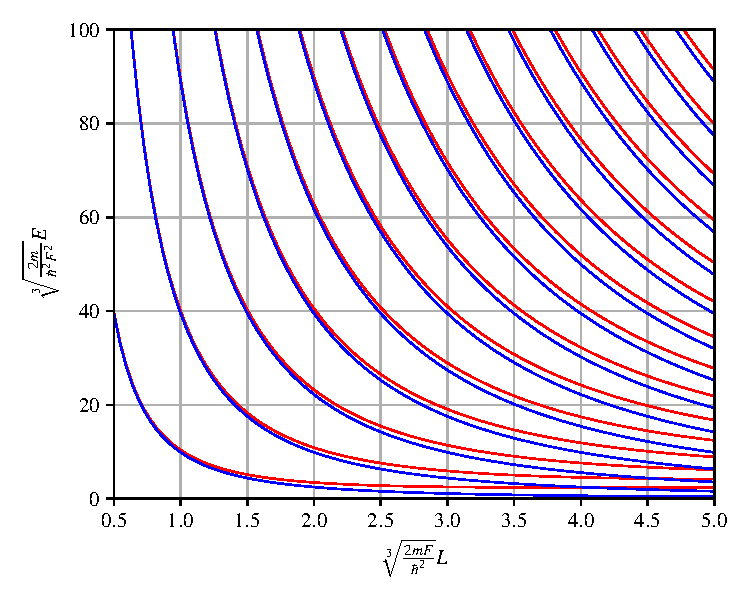
\includegraphics[scale=1]{./figs/infsquareenergia.pdf}
	\caption[Végtelen potenciálgödör energiaszintjei]{Az ábrán a végtelen potenciálgödör és az egzakt energiaszintek összehasonlítása látható. Ez csak az $E \gg FL$ esetben jó közelítés, a szemiklasszikus energiaszintek jóval pontosabbak.}
	\label{semiclassicallevels:squarewell}
\end{figure}